% !TeX root = QuimNadalBargues_CV_Cat.tex
\documentclass[11pt,a4paper]{article}
\usepackage[utf8]{inputenc}
\usepackage[T1]{fontenc}
\usepackage[catalan]{babel}
\usepackage{graphicx}
\usepackage{tabularx}
\usepackage{hyperref}
\usepackage{multirow}
\usepackage{array}
\usepackage{ragged2e}
\usepackage{enumitem}
\usepackage{xcolor}
\usepackage{geometry}
\usepackage{fontawesome5} % Paquet d'icones modern

\geometry{a4paper, left=0.4in, right=0.4in, top=0.25in, bottom=0.25in}

\newcommand{\cvsection}[1]{
    \vspace{0.5em}
    \noindent\textbf{\large #1}
    \vspace{0.5em}
    \hrule\vspace{0.5em}
}
\newcommand{\cvsubsection}[1]{
\vspace{0.3em}
    \noindent\textbf{#1}
    \vspace{0.2em}
}

\newcommand{\skillsep}{\ {\color{gray}\textbar}\ }

\begin{document}

\noindent
\begin{minipage}{0.25\textwidth}
    \vspace*{10pt}
    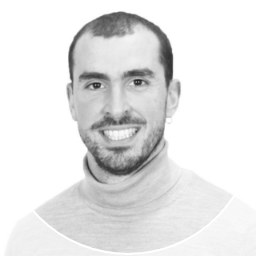
\includegraphics[width=\linewidth,keepaspectratio]{media/ProfilePicture.png} \\
    \cvsection{Contacte}
    \begin{tabular}{@{}ll@{}}
        \faLinkedin & \href{https://www.linkedin.com/in/quimnadalbargues/}{Quim Nadal Bargués} \\
        \faHome & Barcelona, 22/04/1995 \\
        \faPhone & +34 620 200 817 \\
        \faEnvelope & \href{mailto:quimnaba@gmail.com}{quimnaba@gmail.com} \\
    \end{tabular}
    
    \cvsection{Idiomes}
        Castellà (Natiu) \\
        Català (Natiu) \\
        Anglès (C1)
        
    \cvsection{Comp. Tècniques}
        \begin{tabular}{@{}ll@{}}
        \textbf{Llenguatges:}\\
          C\skillsep C++\skillsep Python \\
          Bash\skillsep Java\skillsep VisualBasic\\
          XML\skillsep JSON\skillsep SQL\\
        \textbf{Control:}\\
          Matlab\skillsep Simulink \\
        \textbf{Embedded:}\\
            Lauterbach TRACE32\\ 
            J-Link (Segger)\\
        \textbf{Automoció:}\\
          Vector Tools\\
          ASPICE\skillsep Doors\\
        \textbf{Gestió de Projectes:}\\
        Jira\skillsep Excel\skillsep SVN \\
        \textbf{Competències Generals:} \\
          Git\skillsep Windows\skillsep Linux\\
          CAN\skillsep ETH\skillsep RTP \\
          Android\skillsep Docker\skillsep LaTeX \\
          Enterprise Architect
          \end{tabular}
    
    \cvsection{Comp. Personals}
    \begin{tabular}{@{}ll@{}}
        Humilitat            \\
        Treball en equip    \\
        Presa de decisions     \\
        Pensament lògic    \\
        Tolerància
    \end{tabular}
    
    \cvsection{Interessos}
    \begin{tabular}{@{}ll@{}}
        Esports       \\
        Fotografia  \\
        Viatges\\
        Permisos de conduir: \\
        A, A2, A1, AM, B \\
    \end{tabular}
\end{minipage}
\hfill
\begin{minipage}[t]{0.68\textwidth}
    \vspace*{-26\baselineskip}
    \nointerlineskip
    \begin{flushleft}
        {\fontsize{22}{0}\selectfont\bfseries Quim Nadal Bargués} \\
        \vspace{-8pt}
        \rule{\linewidth}{0.5pt} \\
        \vspace{4pt}
        {\large\bfseries Enginyer de Telecomunicacions | Desenvolupador de Software}
    \end{flushleft}
    
    % Resum Professional
    \cvsection{Perfil Professional}
    Enginyer de Telecomunicacions amb 6+ anys d'experiència, especialitzat en sistemes electrònics de control, software d'aplicació i sistemes incrustats, treballant amb aplicacions d'alt rendiment. Experiència demostrada en tot el procés de desenvolupament: definició de requisits, disseny, implementació i validació. Amb experiència en col·laboració internacional i optimització de rendiment.
   
    \cvsection{Experiència Professional}
    \noindent
    \textbf{Enginyer de Software} \hfill \textbf{Nov 2021 - Actualitat} \\
    \textit{Creadis S.A | Sector Energia Eòlica} \hfill \textit{(Barcelona - Híbrid)}
    
    Desenvolupament d'aplicacions electròniques de control crític per a sistemes de software de turbines eòliques, per a les empreses Vestas i Siemens Energy, passant per totes les fases de desenvolupament. Tot gestionant el processament de dades en temps real de més de 200 sensors, els seus paràmetres, alarmes... \\
    Assoliments clau:
    \begin{itemize}[leftmargin=*,topsep=2pt,itemsep=-1pt]
        \item Redisseny del subsistema de lubricació mitjançant principis POO, permetent el control coordinat de varies bombes de lubricació (millora de funcionalitat i rendiment).
        \item Desenvolupament d'un algorisme de control electrònic per compensar sensors ambientals defectuosos mitjançant integració en temps discret.
    \end{itemize}
    
    \noindent
    \textbf{Enginyer de Software} \hfill \textbf{Feb 2018 - Nov 2021} \\
    \textit{Ficosa S.L | Sector Automoció} \hfill \textit{(Barcelona)} \vspace{4pt}
    
    Desenvolupament d'aplicacions crítiques en C per a sistemes d'assistència en l'aparcament del Grup Volkswagen.\\ Contribucions destacables:
    \begin{itemize}[leftmargin=*,topsep=2pt,itemsep=-1pt]
        \item Disseny de l'algorisme de software d'aplicació per a la calibració d'una càmera de visió posterior (C) complint tots els requisits funcionals.
        \item Documentació arquitectònica completa del sistema de càmera de visió posterior.
        \item Contribució al disseny i especificació de requisits del sistema de càmera de visió superior.
        \item Depuració de problemes complexos analitzant traces de trànsit CAN, Ethernet i RTP.
        \item Desenvolupament d'una eina Python per a la Gestió Automatitzada de Projectes (90\% més ràpid en planificació)
    \end{itemize}
    
    % Educació
    \cvsection{Formació}
    \noindent
    \textbf{Màster en Enginyeria Informàtica} \hfill \textbf{2023 - Actualitat (Previst 2026)} \\
    \textit{Universitat Oberta de Catalunya} \hfill \textit{Barcelona (Remot)} \\
    Especialització: Sistemes de Software Avançats i Computació Distribuïda.\\
    Compatibilitzant amb treball professional a temps complet.\\
    Assignatures rellevants: Arquitectura al núvol, Intel·ligència Artificial, Ciberseguretat.\\
    \noindent
    \textbf{Màster en Enginyeria de Telecomunicacions} \hfill \textbf{2013 - 2018} \\
    \textit{Universitat Politècnica de Catalunya} \hfill \textit{Barcelona}\\
    Especialitat: Sistemes Electrònics. Treball final sobre l'eina d'automatització de PM a Ficosa.\\    
\end{minipage}
\hspace{0.02\textwidth}

\end{document}